

\section{Prueba 4}

\subsection{Red de inferencia}
\begin{center}
	\tikzstyle{regla}= [rectangle,draw,black,fill=blue!15]
	\tikzstyle{hecho}= [rectangle,draw,black,fill=black!15]
	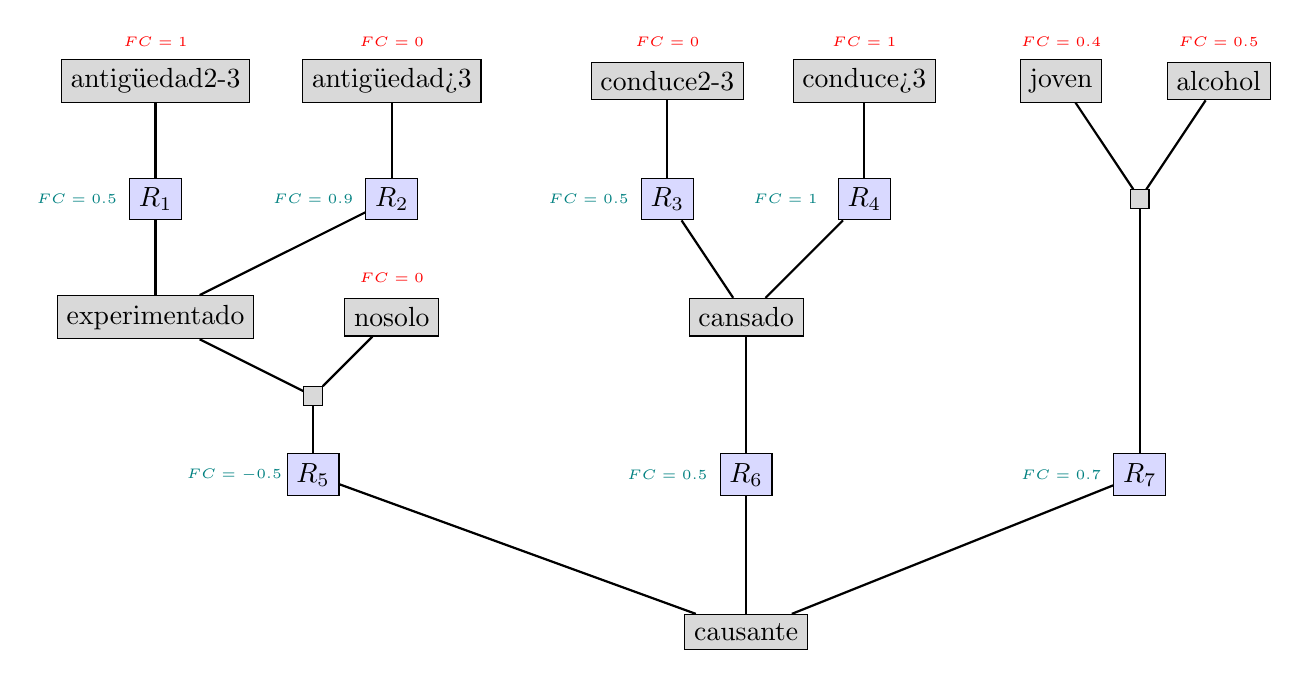
\begin{tikzpicture}
		
		\node (a) at (-3,5) [hecho] {antigüedad2-3};
		\node at (-3,5.5) {\color{red}{\tiny{$FC=1$}}};

		\node (b) at (0,5) [hecho] {antigüedad>3};
		\node at (0,5.5) {\color{red}{\tiny{$FC=0$}}};

		\node (c) at (3.5,5) [hecho] {conduce2-3};
		\node at (3.5,5.5) {\color{red}{\tiny{$FC=0$}}};

		\node (d) at (6,5)[hecho] {conduce>3};
		\node at (6,5.5) {\color{red}{\tiny{$FC=1$}}};

		\node (e) at (-3,2)[hecho] {experimentado};
		
		\node (f) at (4.5,2)[hecho] {cansado};

		\node (g) at (8.5,5)[hecho] {joven};
		\node at (8.5,5.5) {\color{red}{\tiny{$FC=0.4$}}};

		\node (h) at (10.5,5)[hecho] {alcohol};
		\node at (10.5,5.5) {\color{red}{\tiny{$FC=0.5$}}};

		\node (i) at (0,2)[hecho] {nosolo};
		\node at (0,2.5) {\color{red}{\tiny{$FC=0$}}};

		\node (j) at (4.5,-2)[hecho] {causante};

		\node (e/i) at (-1,1)[hecho] {};
		\node (g/h) at (9.5,3.5)[hecho] {};

		\node (r1) at (-3,3.5) [regla] {$R_{1}$};
		\node at (-4,3.5) {\color{teal}{\tiny{$FC=0.5$}}};
		\node (r2) at (0,3.5) [regla] {$R_{2}$};
		\node at (-1,3.5) {\color{teal}{\tiny{$FC=0.9$}}};
		\node (r3) at (3.5,3.5) [regla] {$R_{3}$};
		\node at (2.5,3.5) {\color{teal}{\tiny{$FC=0.5$}}};
		\node (r4) at (6,3.5) [regla] {$R_{4}$};
		\node at (5,3.5) {\color{teal}{\tiny{$FC=1$}}};
		\node (r5) at (-1,0) [regla] {$R_{5}$};
		\node at (-2,0) {\color{teal}{\tiny{$FC=-0.5$}}};
		\node (r6) at (4.5,0) [regla] {$R_{6}$};
		\node at (3.5,0) {\color{teal}{\tiny{$FC=0.5$}}};
		\node (r7) at (9.5,0) [regla] {$R_{7}$};
		\node at (8.5,0) {\color{teal}{\tiny{$FC=0.7$}}};

		\path[black,thick] (a) edge[] node {} (r1);
		\path[black,thick] (r1) edge[] node {} (e);
		\path[black,thick] (b) edge[] node {} (r2);
		\path[black,thick] (r2) edge[] node {} (e);
		\path[black,thick] (e) edge[] node {} (e/i);
		\path[black,thick] (i) edge[] node {} (e/i);
		\path[black,thick] (e/i) edge[] node {} (r5);
		\path[black,thick] (r5) edge[] node {} (j);
	
	
		\path[black,thick] (c) edge[] node {} (r3);
		\path[black,thick] (r3) edge[] node {} (f);
		\path[black,thick] (d) edge[] node {} (r4);
		\path[black,thick] (r4) edge[] node {} (f);
		\path[black,thick] (f) edge[] node {} (r6);
		\path[black,thick] (r6) edge[] node {} (j);

		\path[black,thick] (g) edge[] node {} (g/h);
		\path[black,thick] (h) edge[] node {} (g/h);
		\path[black,thick] (g/h) edge[] node {} (r7);
		\path[black,thick] (r7) edge[] node {} (j);

	\end{tikzpicture}
\end{center}

\subsection{Objetivo obtenido por SBR-FC}

\subsection{Cuestión}
\begin{ejer}
	\textbf{Prueba 4.} Un \texttt{conductor} de 32 años (entendemos que es joven con grado 0.4), 
	con 2-3 años de antigüedad, ha conducido durante más de 3 horas, viajaba solo y 
	había bebido algo de alcohol (entendemos que su factor de certeza es de 0.5). \\
	¿Cuál será el grado de certeza de que este conductor ha sido causante del accidente?
\end{ejer}